\section{Нерекурсивный фильтр}
\label{sec:nerekurs}

\subsection{Расчёт фильтра}

\point Расчёт цифрового фильтра высоких частот (ФВЧ) со строго
линейной ФЧХ выполняется \textit{методом взвешивания}. Данный метод не
позволяет синтезировать оптимальные фильтры, но гораздо более удобен
для расчётов и даёт вполне приемлемые для практики результаты [1].


\point Исходные данные:

\begin{itemize}
\item тип фильтра~--- ФВЧ;
\item затухания в полосе задержания $a_0 = 45$ дБ;
\item характерные частоты фильтра $f_1 = 3000$ Гц;
\item ширина переходной полосы $\Delta f = 900$ Гц;
\item частота дискретизации $f_{\text{\textit{д}}} = 8000$ Гц;
\item мощность выходного шума квантования
    $\sigma^2_{\text{\textit{вых}}} = 5 \cdot 10^{-6}$.
\end{itemize}


\point Для упрощения обозначений удобно использовать нормализованную
шкалу относительных (или нормированных) частот:

\begin{equation}
  \label{eq:otn_freq}
  f_0 = \frac{f}{f_{\text{д}}},
\end{equation}

\begin{ESKDexplanation}
\item[где ] $f_{\text{д}}$~--- частота дискретизации;
\item $f_0$~--- относительное значение частоты;
\item $f$~--- абсолютное значение частоты.
\end{ESKDexplanation}

Таким образом, по формуле~(\ref{eq:otn_freq}):

\begin{gather*}
  f_{01} = \frac{f_1}{f_{\text{д}}} = \frac{3000}{8000} = 0{,}375;\\
  \Delta f_0 = \frac{\Delta f}{f_{\text{д}}} = \frac{900}{8000} = 0{,}113.
\end{gather*}


\point В соответствии с заданной величиной затухания в полосе
задерживания $a_0 = 45$ и графиками для окна Ланцоша, определяется
положительная постоянная~$L$ (см. формулу~(\ref{eq:lancosh})) и
\textit{порядок фильтра}~$N$:

\begin{gather*}
  (N-1)\Delta f_0 = 3;\\
  N = 27;\\
  L = 1{,}5.
\end{gather*}


\point \textit{Коэффициенты разложения в ряд Фурье} идеальной АЧХ
фильтра верхних частот:

\begin{gather}
  \nonumber
  h(0) = 1 - 2f_{01};\\
  \label{eq:koef_furier}
  h(k) = - \frac{\sin(2 \pi k f_{01})}{k \pi}.\\
  \nonumber
  k = - \frac{N}{2}, \ldots , \frac{N}{2} = -13, \ldots, 13.
\end{gather}

Результаты вычислений занесены в таблицу~\ref{tab:nonrekurs}
приложения~\ref{sec:AppendixA}.


\point Для уменьшения амплитуды пульсаций усечение импульсной реакции
производят с использованием весовой последовательности конечной длинны
$w(k)$, называемой временным окном. \textit{Весовые множители} $w(k)$
вычисляются из следующего выражения:

\begin{gather}
  \label{eq:lancosh}
  w(k) = \left[\frac{\displaystyle\sin\left(\frac{2\pi
          k}{N-1}\right)}{\displaystyle\frac{2\pi k}{N-1}}\right]^L,\\
  \nonumber
  k = -13, \ldots, 13,\\
  \nonumber
  L = 1{,}5.
\end{gather}

Результаты вычислений занесены в таблицу~\ref{tab:nonrekurs}
приложения~\ref{sec:AppendixA}.


\point На следующем этапе необходимо вычислить \textit{коэффициенты
  фильтра}. Процедура взвешивания сводится к умножению отсчётов $h(k)$
на соответствующие отсчёты $w(k)$ временного окна. Поэтому
коэффициенты ФВЧ вычисляются по формуле:

\begin{equation*}
  \hat h(k) = h(k) \cdot w(k).
\end{equation*}

Вычисленные значения коэффициентов фильтра представлены в
таблице~\ref{tab:nonrekurs} приложения~\ref{sec:AppendixA}.


\point Далее рассчитывается \textit{разрядность коэффициентов
  фильтра}. Коэффициенты каузального (физически реализуемого) фильтра
должны быть представимы конечным числом двоичных разрядов $N_k$.
Значение $N_K$ можно рассчитать по формуле:

\begin{align}
  \nonumber N_K & = \left[\log_2\left(\displaystyle
      \frac{\displaystyle 10 \cdot \frac{a_0}{20} \cdot
        \sqrt{\frac{2N-1}{3}}}{2}\right) \right]_{\text{Ц.Ч.}} + 1 =\\
  \nonumber & = \left[\log_2\left(\displaystyle \frac{\displaystyle 10
        \cdot \frac{45}{20} \cdot \sqrt{\frac{2 \cdot
            27-1}{3}}}{2}\right) \right]_{\text{Ц.Ч.}} + 1 = 7.
\end{align}


\point Далее по формуле~(\ref{eq:koef_okr}) вычисляются
\textit{округлённые значения коэффициентов фильтра}. Результаты
округления значений фильтра сведены в таблицу~\ref{tab:nonrekurs}
приложения~\ref{sec:AppendixA}.

\begin{equation}
  \label{eq:koef_okr}
  h_{\text{окр}} = 2^{-N_K} \cdot \left[h \cdot 2^{N_K}\right]_{\text{Ц.Ч.}}.
\end{equation}


\point Для практической реализации фильтра необходимо также оценить
\textit{разрядность входного} $S_{\text{вх}}$ и \textit{выходного}
$S_{\text{вых}}$ \textit{регистров фильтра}. Эти величины определяют
параметры шума квантования. Для определения величин $S_{\text{вх}}$ и
$S_{\text{вых}}$ можно пользоваться формулами:

\begin{gather*}
  S_{\text{вх}} = \left[ 0{,}5 \cdot \log_2\left(\frac{1{,}1 \sum_{l
          =0}^{N-1} \hat h^2(l)}{12 \sigma^2_{\text{вых}}} \right)
  \right]_{\text{Ц.Ч.}}
  + 1;\\
  S_{\text{вых.д}} = \left[0{,}5 \cdot \log_2\left( \frac{12N}{12
        \sigma^2_{\text{вых}} -2^{-2S_{\text{вх}}} \sum_{l=0}^{N-1}
        \hat
        h^2(l)}\right)\right]_{\text{Ц.Ч.}} + 1;\\
  S_{\text{вых.ц.}} = \left[0{,}5 \log_2 \sum_{l=0}^{N-1} \left|\hat
      h(l)\right|\right]_{\text{Ц.Ч.}};\\
  S_{\text{вых}} = S_{\text{вых.д}} + S_{\text{вых.ц.}}.
\end{gather*}

Выполнив необходимые вычисления, получаем:

\begin{gather*}
  S_{\text{вх}} = 7, \quad
  S_{\text{вых.д}} = 12,\quad
  S_{\text{вых.ц.}} = 0;\\
  S_{\text{вых}} = 12 + 0 = 12.
\end{gather*}

\subsection{АЧХ фильтра}

Комплексную частотную характеристику (КЧХ) нерекурсивного цифрового
фильтра можно определить из следующего соотношения:

\begin{equation*}
  H(e^{j\omega_0}) = \sum_{K=0}^{N-1}h(k) \cdot e^{-j\omega_0k},
\end{equation*}

\begin{ESKDexplanation}
\item[где ] $\omega_0$~--- круговая нормированная частота;
\item $N$~--- порядок фильтра.
\end{ESKDexplanation}

АЧХ представляет собой абсолютное значение от КЧХ. Модуль комплексного
числа можно определить как квадратный корень из суммы квадратов
вещественной и мнимой частей:

\begin{equation*}
\left|H(e^{j\omega_0}) \right| = \sqrt{\text{Re}^2H(e^{j\omega_0k}) + \text{Im}^2H(e^{j\omega_0k})}.
\end{equation*}

Используя формулу Эйлера:

\begin{equation*}
  e^{j\omega_0} = \cos\omega_0 + j \sin\omega_0,
\end{equation*}

записывается конечная формула для расчёта АЧХ нерекурсивного фильтра.

\begin{equation*}
   \left|H(e^{j\omega_0})\right| = \sqrt{\left[\sum_{k =
        -\frac{N-1}{2}}^{k =
        \frac{N-1}{2}}h(k)\cos(k\omega_0)\right]^2 + \left[\sum_{k =
        -\frac{N-1}{2}}^{k =
        \frac{N-1}{2}}h(k)\sin(k\omega_0)\right]^2}.
\end{equation*}

Для вычисления АЧХ нерекурсивного фильтра, необходимо оценить её на
главном значении периода. Для этого вычисляется дискретное
преобразование Фурье (ДПФ) этой функции.

\begin{figure}[h!]
  \label{f:1}
  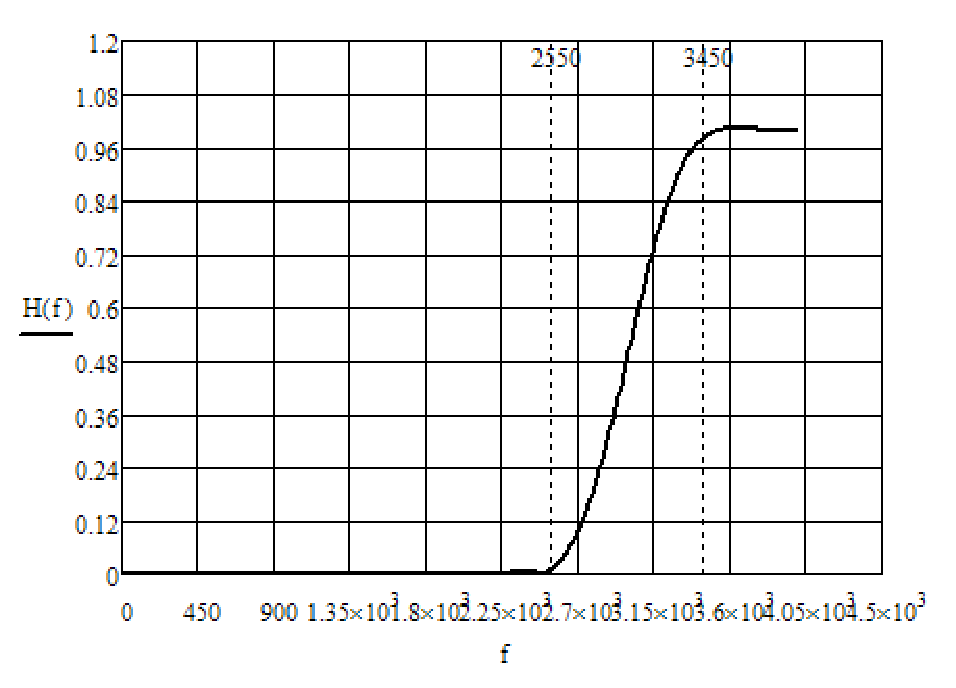
\includegraphics{nerekurs_ach}
  \caption{АЧХ синтезированного нерекурсивного фильтра верхних частот}
\end{figure}

Для более удобного сопоставления полученных частотных характеристик с
требованиями технического задания, целесообразно значения АЧХ выразить
в логарифмических единицах:

\begin{equation*}
  a_0 = -20 \lg\left|H(e^{j \omega_0})\right|.
\end{equation*}

Для получения требуемой характеристики величина $N$ была увеличена до 14.

\begin{figure}[h!]
  \label{f:2}
  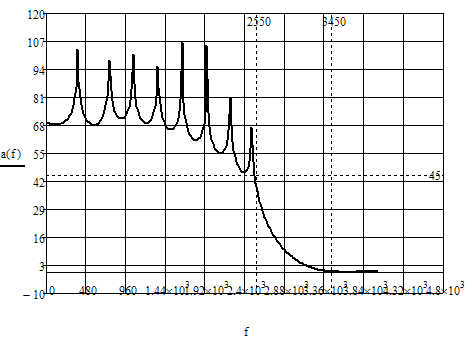
\includegraphics{nerekurs_lach}
  \caption{ЛАЧХ синтезированного фильтра}
\end{figure}


Из графика представленного на рисунке~\ref{f:2} видно, что АЧХ синтезируемого
фильтра удовлетворяет требованиям технического задания. Это следует из
того, что на частоте 2550 Гц затухание соответствует 45 дБ.

\subsection{Структурная схема фильтра}

Структурная схема нерекурсивного цифрового фильтра приведена на 
рисунке~\ref{nerekurs_dia}.

\begin{figure}[h!]
  \label{nerekurs_dia}
  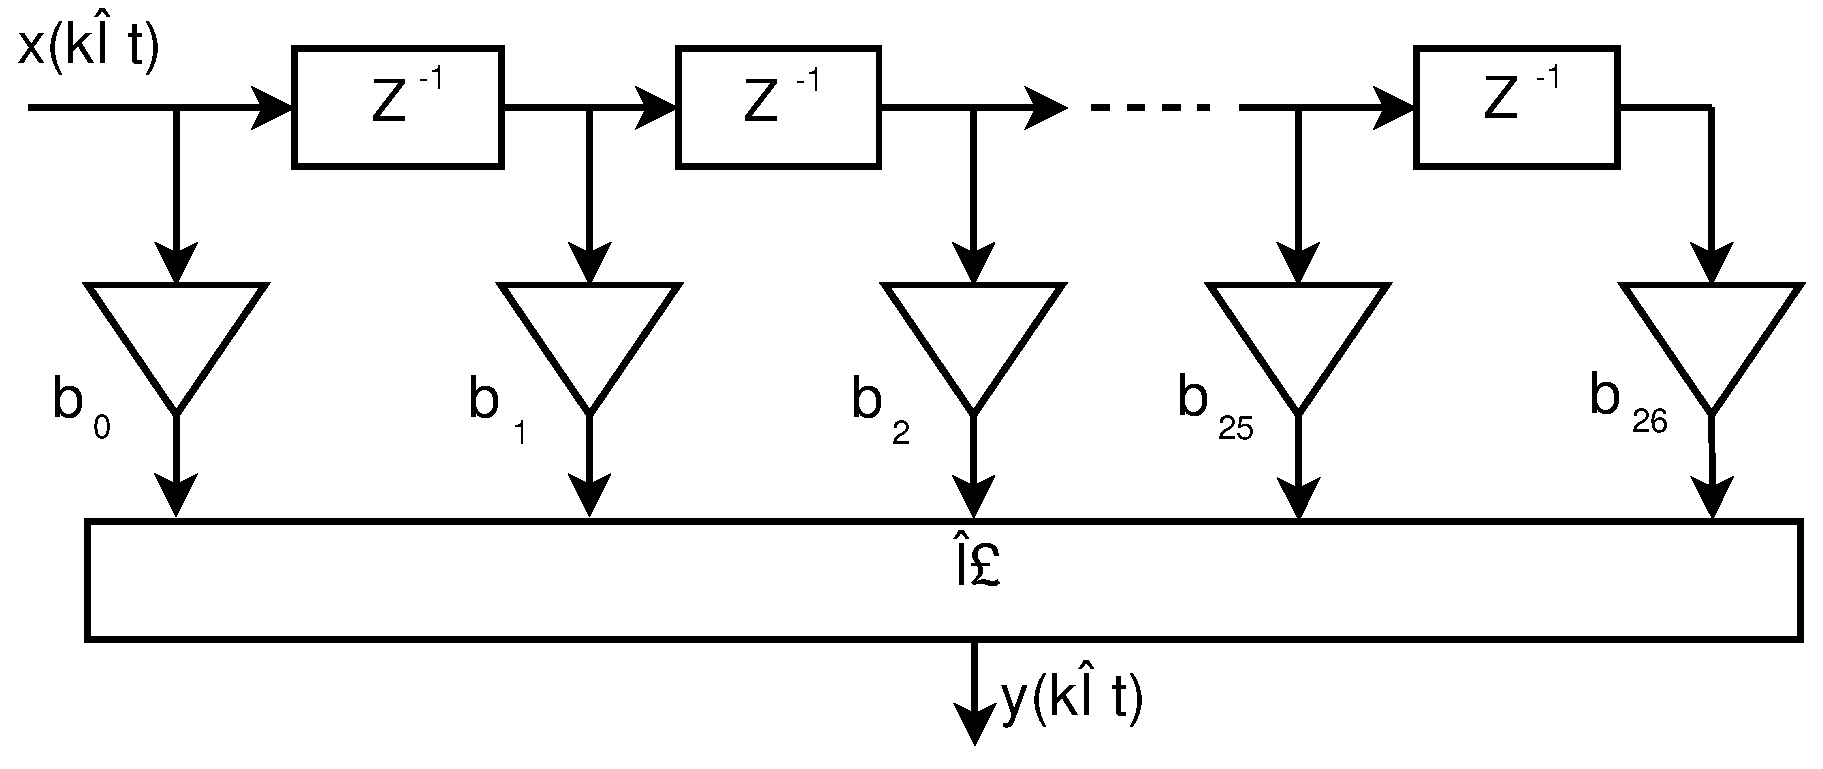
\includegraphics[width=\textwidth]{nerekurs}
  \caption{Структурная схема нерекурсивного фильтра}
\end{figure}

\newpage

\section{Рекурсивный фильтр}
\label{sec:rekurs}

\subsection{Расчёт фильтра}

\point Наиболее распространённым и простым методом синтеза для
стандартных частотно-избирательных фильтров является \textit{метод билинейного
преобразования} передаточной функции $K(P)$ аналогового фильтра-прототипа
(АФ) в соответствующую передаточную функцию $H(z)$ цифрового
рекурсивного фильтра (ЦРФ) [1].

\point Исходные данные:

\begin{itemize}
\item тип фильтра, характер аппроксимации~--- ППФ, Чебышева;
\item затухание в полосе задержания $a_0 = 40$ дБ;
\item верхняя граница затухания в полосе пропускания $\Delta a =$~0{,}8~дБ;
\item характерные частоты фильтра $f_{11} = 900$ Гц, $f_{12} = 1800$
  Гц, $f_{21} = 500$ Гц, $f_{22} = 2200$ Гц;
\item частота дискретизации $f_{\text{\textit{д}}} = 4800$ Гц;
\item мощность выходного шума квантования
  $\sigma^2_{\text{\textit{вых}}} = 10^{-5}$.
\end{itemize}

\point Согласно формуле~(\ref{eq:otn_freq}) \textit{относительные значения
характерных частот} фильтра:

\begin{gather*}
  f_{011} = 0{,}1875;\\
  f_{012} = 0{,}3750;\\
  f_{021} = 0{,}1042;\\
  f_{022} = 0{,}4583.
\end{gather*}

\point По формулам, описывающим обобщённое билинейное преобразование,
определяются значения параметров $\gamma$ и $\alpha$, а также
\textit{граничная частота} $\Omega_k$ нормированного аналогового
фильтра-прототипа:

\begin{gather*}
  \gamma = \ctg \left[\pi (f_{012} - f_{011})\right] = 1{,}947;\\
  \alpha = \frac{\cos\left[\pi (f_{012} + f_{011})
    \right]}{\cos\left[\pi (f_{012} - f_{011}) \right]} = -0{,}235;\\
  \Omega'_k = \gamma \frac{\alpha - cos(2\pi f_{021})}{\sin(2\pi
    f_{021})} = -2{,}527;\\
  \Omega''_k = \gamma \frac{\alpha - cos(2\pi f_{022})}{\sin(2\pi
    f_{022})} = 4{,}229;\\
  \Omega_k = \text{min}\bigl(|\Omega'_k|,|\Omega''_k|\bigr) = 2{,}527.
\end{gather*}


\point Следующим этапом является определение \textit{передаточной
  функции} \emph{аналогового фильтра-прототипа} для полосового фильтра
с аппроксимацией Чебышева по справочнику [3]. С помощью справочника
определяем:

\begin{itemize}
\item модуль коэффициента отражения $|P| = 25\%$;
\item вспомогательный параметр $L = 0{,}05$;
\item \textit{порядок фильтра} $n = 5$.
\end{itemize}

В соответствии с данными параметрами \textit{функция фильтрации} для
фильтра-прототипа ППФ с характеристиками Чебышева выглядит следующим
образом:

\begin{equation*}
  S(p) = C(p-a_0)\prod_1^2(p^2-2a_is+a^2_i+b^2_i).
\end{equation*}

\begin{ESKDexplanation}
\item[где ] $C = 4{,}1311822$;
\item $a_0 = 0{,}4245017665$;
\item $a_1 = 0{,}3434291432$;
\item $a_2 = 0{,}1311782600$;
\item $b_1 = 0{,}6385527983$;
\item $b_2 = 1{,}0332001312$.
\end{ESKDexplanation}

Передаточная функция:

\begin{equation}
  \label{eq:pered}
  K(p) = \frac{1}{S(p)} = \frac{1}{C(p-a_0)\prod_1^2(p^2-2a_is+a^2_i+b^2_i)}.
\end{equation}

\point Чтобы избежать трудоёмкого расчёта уравнения 4-го порядка,
разложили передаточную функцию фильтра-прототипа в виде произведений
полиномов 1-го порядка по степеням $P$ [2]:

\begin{equation}
  \label{eq:poly_proizv}
  P^2 + a_1P + a_2 = (P - P_1)(P - P_2).
\end{equation}

Осуществляя подстановку соответствующих $a$ и $b$, в
знаменателе~(\ref{eq:pered}) сформируются два квадратных уравнения:

\begin{gather*}
  P^2 - 2a_1P + a_1 + b_1 = 0;\\
  P^2 - 2a_2P + a_2 + b_2 = 0.
\end{gather*}

В результате решения квадратных уравнений были получены следующие
корни:

\begin{gather*}
  p_1 = 0{,}343 - 0{,}639i;\\
  p_2 = 0{,}343 + 0{,}639i;\\
  p_3 = 0{,}131 - 1{,}033i;\\
  p_4 = 0{,}131 + 1{,}003i.\\
  p_5 = 0{,}4245.
\end{gather*}

Используя~(\ref{eq:poly_proizv}), (\ref{eq:pered}) преобразуется в
вид:

\begin{equation}
  \label{eq:pered_proizv_poly}
  K(p) = \frac{A}{\prod_{i=0}^{n-1}(p-p_i)},
\end{equation}

\begin{ESKDexplanation}
\item[где ] $A = \frac{1}{C} = 0{,}2421$;
\item $n = 5$.
\end{ESKDexplanation}

\point Следующим этапом является определение \textit{передаточной
  функции} \emph{цифрового фильтра}. Для перехода от передаточной
функции АФ к передаточной функции ЦФ необходимо использовать функцию
замены для ППФ:

\begin{equation}
  \label{eq:zamena}
  P  \rightarrow \gamma \frac{1 - 2 \alpha z^{-1}+z^{-2}}{1-z^{-2}}.
\end{equation}

Умножая числитель и знаменатель дроби~(\ref{eq:zamena}) на $z^2$ и
подставляя полученное выражение в
формулу~(\ref{eq:pered_proizv_poly}), получаем выражение для
\textit{передаточной функции}:

\begin{equation*}
  H(z) = \frac{A(z^2-1)^n}{\displaystyle \prod_{i=0}^{n-1}\left[(\gamma - p_i)z^2 - 2
      \alpha \gamma z + (\gamma + p_i)\right]}.
\end{equation*}

\point Значения полюсов:

\begin{align*}
  z_{1}= -0{,}712 - 0{,}956i;\\
  z_{2}= 0{,}246 + 1{,}215i;\\
  z_{3}= -0{,}712 + 0{,}956i;\\
  z_{4}= 0{,}246 - 1{,}215i;\\
  z_{5}= -0{,}756 - 0{,}733i;\\
  z_{6}= 0{,}429 + 0{,}980i;\\
  z_{7}= -0{,}756 + 0{,}733i;\\
  z_{8}= 0{,}429 - 0{,}980i;\\
  z_{9}= 0{,}328 + 1{,}298i;\\
  z_{10} = -0{,}328 - 1{,}298i
\end{align*}

\point Для того чтобы избавиться от комплексных коэффициентов, нужно
представить каждый из полиномов в виде:

\begin{equation*}
  az^2 + A_2z + A_3 = a(z-z_i)(z-z_j),
\end{equation*}

\begin{ESKDexplanation}
\item[где ] $z_i$, $z_j$~--- комплексные корни квадратных уравнений
  вида: $az^2 + A_2z + A_3 = 0$;
\item $a = (\gamma - p_i)$;
\item $A_2 = - 2 \alpha \gamma$;
\item $A_3 = (\gamma + p_i)$.
\end{ESKDexplanation}

Затем, перемножив сомножители вида $(z - z_i)$ и $(z- z_j^*)$, где
$z_j^*$~--- комплексно-сопряженное с $zi$, получаются полиномы второго
порядка относительно $z$ с действительными коэффициентами.

\begin{gather*}
  \prod_{i=1}^{5}a_i = \prod_{i=1}^{5}(\gamma - p_i) = k = 5{,}462.\\
  (z - z_1)(z - z_3)   = z^2 + 1{,}424z + 1{,}422;\\
  (z - z_2)(z - z_4)   = z^2 - 0{,}492z + 1{,}536;\\
  (z - z_3)(z - z_5)   = z^2 + 1{,}512z + 1{,}108;\\
  (z - z_6)(z - z_8)   = z^2 - 0{,}857z + 1{,}144;\\
  (z - z_9)(z - z_{10}) = z^2 + 0{,}655z + 1{,}792.\\
  v = \frac{A}{k} = 0{,}044.
\end{gather*}

\textit{Коэффициенты фильтра} имеют вид:

\begin{align*}
  a_1& =    1{,}424; & b_1 =  1{,}422;\\ 
  a_2& =  - 0{,}492; & b_2 =  1{,}536;\\ 
  a_3& =    1{,}512; & b_3 =  1{,}108;\\ 
  a_4& =  - 0{,}857; & b_4 =  1{,}144;\\ 
  a_5& =    0{,}655; & b_5 =  1{,}792.\\ 
\end{align*}

\point Для того, чтобы получить выражение для \textit{передаточной
  функции} синтезируемого фильтра в \emph{каноническом виде}
(содержащем в числителе и знаменателе полиномы по отрицательным
степеням $z$), необходимо разделить числитель и знаменатель дроби на
$z^2$. Искомая передаточная функция:

\begin{equation}
  \label{eq:pered_kanon}
  H(z) = \frac{v(1 - z^{-2})^5}{\prod_{i=1}^5\left(1 + a_i z^{-1} +b_i
    z^{-2}\right)}.
\end{equation}

\point Далее необходимо оценить \textit{разрядность входного регистра}
фильтра с помощью формулы:

\begin{equation}
  \label{eq:rekurs_razr}
  S_{\text{вх}} = \left[0{,}5 \log_2 \frac{\displaystyle
      \sum_{n=0}^{\infty} \bigl(h(n)\bigr)^2}{12
      \sigma^2_{\text{вых}}}\right]_{\text{ц.ч.}} + 1,
\end{equation}

\begin{ESKDexplanation}
\item[где ] $\sigma^2_{\text{вых}}$~--- допустимая мощность шума
  квантования;
\item $h(n)$~--- $n$-ый отсчёт импульсной реакции РЦФ.
\end{ESKDexplanation}

Необходимое значение $\sum_{n=0}^{\infty} \bigl(h(n)\bigr)^2$ можно
вычислить с помощью равенства Парсеваля:

\begin{equation}
  \label{eq:parsev}
  \sum_{n = -\infty}^{\infty}\bigl(h(n)\bigr)^2 = \frac{1}{2 \pi j}
  \oint_{C} H(z) H(z^{-1}) z^{-1} \, dz,
\end{equation}

\begin{ESKDexplanation}
\item[где ] $H(z)$~--- передаточная функция синтезированного фильтра.
\end{ESKDexplanation}

Контурный интеграл в выражении~(\ref{eq:parsev}) может быть вычислен с
помощью теоремы и вычетах [1], которая звучит так:

\begin{quote}
  \textit{Интеграл по замкнутому контуру от функции $f(z)$ равен сумме вычетов в
  полюсах $f(z)$, схваченных этим контуром, умноженной на $2\pi i$, то есть:}
\end{quote}

\begin{equation}
  \label{eq:kont_int}
  \oint_{C}f(z) \, dz = 2\pi i \sum_{i=1}^{L}
  \text{Res}\bigl((x)r\bigr)\Big|_{z = P_i \in C},
\end{equation}

\begin{ESKDexplanation}
\item[где ] $L$~--- число полюсов комплексного переменного;
\item $P_i$~--- полюс кратности $m$;
\item а вычет от функции $f(z)$ в точке $z = P_i$ определяется по формуле:
\end{ESKDexplanation}

\begin{gather*}
  \text{Res}\bigl(f(z)\bigr)\Big|_{z=P_i} = \frac{1}{(m-1)!} \lim
  \limits_{z \rightarrow P_i}
  \frac{d^{m-1}}{dz^{m-1}}\bigl((z-P_i)^mf(z)\bigr) \\
  \text{(для кратных полюсов)}.\\
  \text{Res}\bigl(f(z), z_0\bigr) = \lim f(z)(z-z_0) \\
  \text{(для простых полюсов)}.\\
\end{gather*}

После проведения всех вычислений, находим $S_{\text{вх}}$= 10. Полученное
значение даёт представление о необходимой разрядности регистров в
реализуемом рекурсивном цифровом фильтре. Точное вычисление количества
разрядов выходного регистра ещё более сложно и не всегда необходимо,
поскольку для реализации цифровых фильтров обычно используют либо
микропроцессоры, либо оперативно-запоминающее устройство с
фиксированной длинной кодового слова~[1].

\subsection{АЧХ фильтра}

Для рекурсивного фильтра комплексная частотная характеристика (КЧХ)
получается путем подстановки $z = e^{j\omega_0}$ в выражение для
$H(z)$~(\ref{eq:pered_kanon}).

Осуществляем подстановку с учётом того, что

\begin{equation*}
  \omega_o = 2\pi\frac{f}{f_{\text{д}}}.
\end{equation*}

\begin{equation*}
  H(z) = \frac{v(1 -
    \left[e^{j\omega_0}\right]^{-2})^5}{\prod_{i=1}^5\left(1 + a_i
      \left[e^{j\omega_0} \right]^{-1} +b_i
      \left[e^{j\omega_0}\right]^{-2}\right)}.
\end{equation*}

Суммарная АЧХ определяется как модуль КЧХ. График АЧХ представлен на
рисунке~2.1. Построение АЧХ производится на главном
значении периода функции $H(e^{j \omega_0})$, т.~е. на интервале от 0
до $\frac{f_{\text{д}}}{2}$.

\begin{figure}[h!]
  \label{fig:rekurs_ach}
  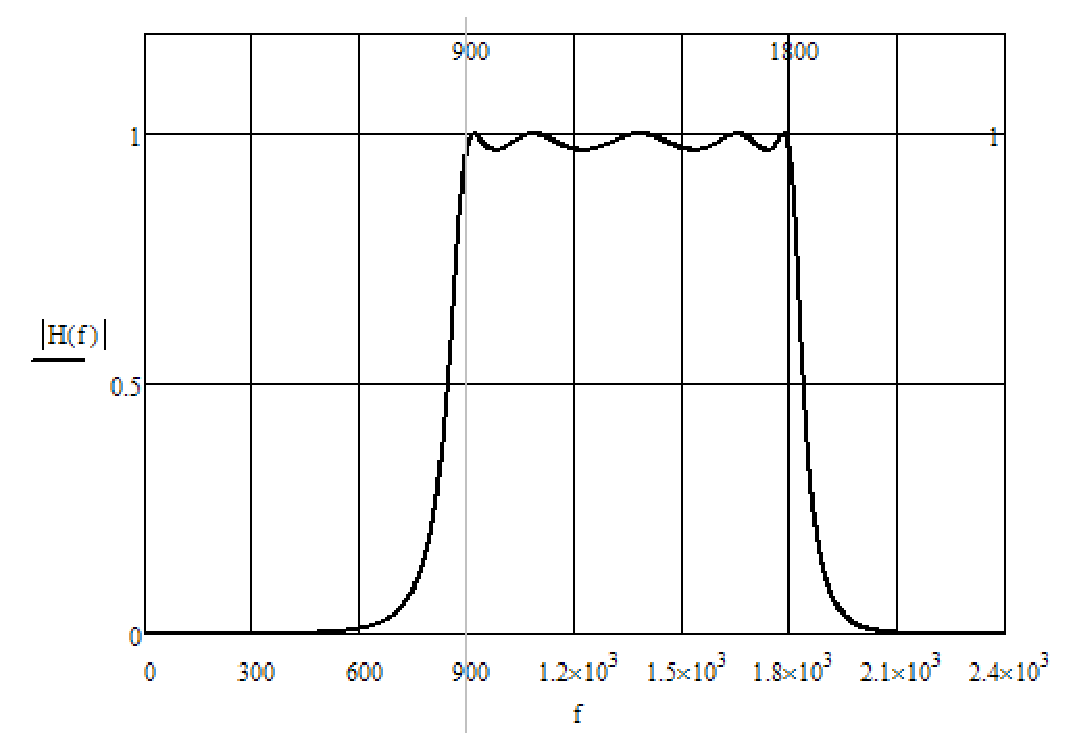
\includegraphics[width=\textwidth]{rekurs_ach}
  \caption{АЧХ синтезированного рекурсивного фильтра}
\end{figure}

Для более удобного сопоставления полученных частотных характеристик с
требованиями технического задания целесообразно значения АЧХ выразить
в логарифмических единицах, то есть определить характеристику
затухания по формуле:

\begin{equation*}
  a_o = -20 \lg\left|H(e^{j\omega_0})\right|.
\end{equation*}

График зависимости затухания от частоты изображён на рисунках~2.2,~2.3.

\begin{figure}[h!]
  \label{fig:zatuh1}
  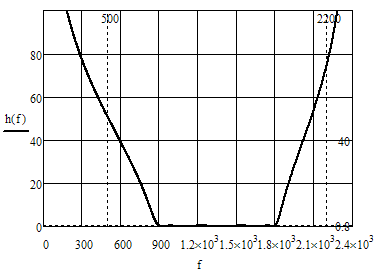
\includegraphics{zatuh1}
  \caption{Зависимость затухания от частоты ($a(f) = 0 \ldots 100$)}
\end{figure}

\begin{figure}[h!]
  \label{fig:zatuh2}
  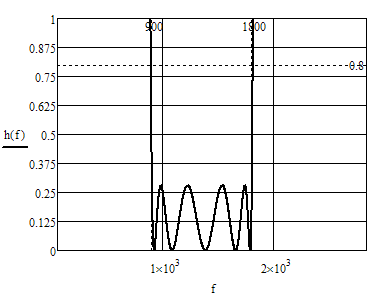
\includegraphics{zatuh2}
  \caption{Зависимость затухания от частоты ($a(f) = 0 \ldots 1$)}
\end{figure}

Согласно требованиям задания, в полосе задержания затухание должно
быть не менее 40~дБ, из графика видно, что это требование
выполнено. Верхняя граница затухания в полосе пропускания не превышает
0{,}8 дБ.

\subsection{Структурная схема фильтра}
\label{sec:scheme_nerekurs}

Структурная схема строится следующим образом. Каждый каскад
передаточной функции $H(z)$ синтезируемого фильтра в каноническом виде
имеет вид:

\begin{equation*}
  H(z) = \frac{b_2z^{-2}+b_1z^{-1}+b_0}{1-a_2z^{-2}-a_1z^{-1}}.
\end{equation*}

Каждый элемент задержки имеет соответствующий коэффициент.
Структурная схема рекурсивного ППФ (каскадная форма) представлена на
рисунке~2.4.

\begin{figure}[p]
  \label{nerekurs_dia}
  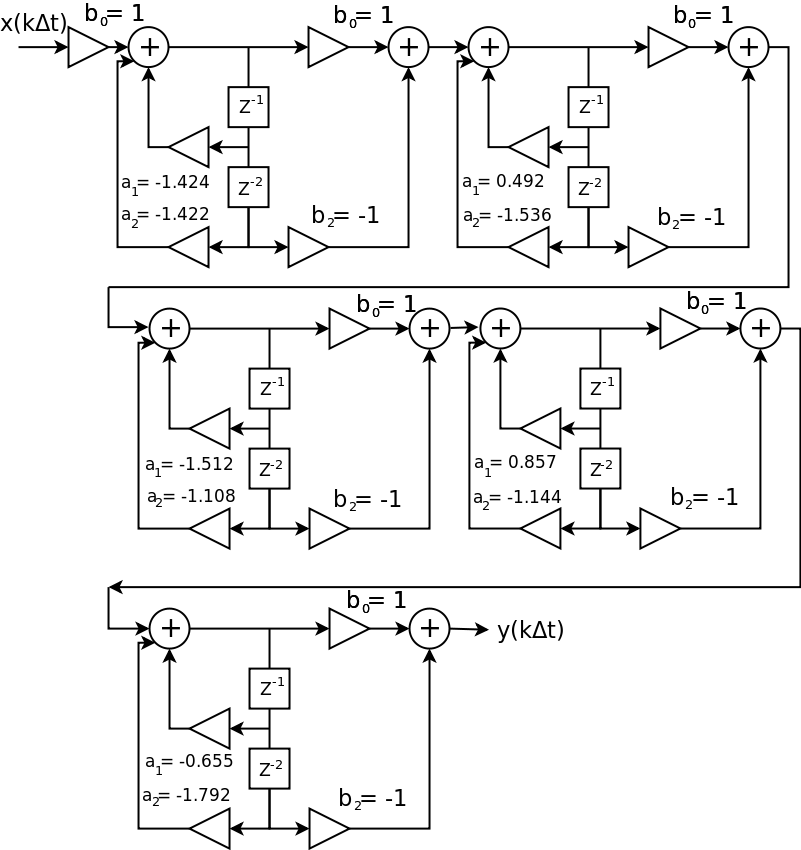
\includegraphics[width=\textwidth]{rekurs}
  \caption{Структурная схема нерекурсивного фильтра}
\end{figure}
\newpage


%%% Local Variables: 
%%% mode: latex
%%% TeX-master: "../TermWork_TES"
%%% End: 
